\subsection{Unlocking the Secrets of Smith Chart Arcs!}

\begin{tcolorbox}[colback=gray!10, colframe=black, title=E9G10]  
What do the arcs on a Smith chart represent?  
\begin{enumerate}[label=\Alph*.]
    \item Frequency
    \item SWR
    \item Points with constant resistance
    \item \textbf{Points with constant reactance}
\end{enumerate} \end{tcolorbox}

In order to understand the question regarding the arcs on a Smith chart, we must first delve into the concepts surrounding impedance matching and transmission lines. The Smith chart is a graphical representation commonly used in radio frequency (RF) engineering to analyze complex impedance and reflection coefficients. Its utility lies in its ability to easily visualize the relationships between impedance, reactance, and standing wave ratio (SWR).

The arcs specifically represent loci of points at a constant value of reactance. In simpler terms, if you were to select a point on the arc, all points on that same arc will have the same reactance (either inductive or capacitive). This is crucial when tuning antennas or matching networks because it allows engineers to easily identify conditions for which the circuit will behave optimally.

To further elucidate this concept, we can look at a portion of the Smith chart in which the horizontal line represents constant resistance while the arcs sloping upwards or downwards from this line represent various levels of reactance. This can be a bit abstract if one is unfamiliar, so let us visualize it with a TikZ diagram.

\begin{center}
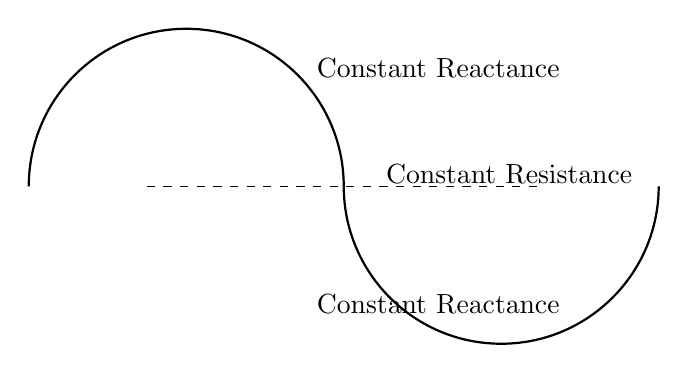
\begin{tikzpicture}
    % Smith chart arc segment
    \draw[thick] (0,0) arc[start angle=0, end angle=180, radius=2cm];
    \draw[thick] (0,0) arc[start angle=180, end angle=360, radius=2cm];
  
    % Constant resistance line
    \draw[dashed] (-2.5,0) -- (2.5,0);
    
    % Labels
    \node at (2.1,0.15) {Constant Resistance};
    \node at (1.2,1.5) {Constant Reactance};
    \node at (1.2,-1.5) {Constant Reactance};
\end{tikzpicture}
\end{center}

To calculate the values represented on the arcs or indicate how they relate to impedance, you would typically use the formulas related to impedance transformation and the equations relating to reactance:
\[
X = \begin{cases} 
j\omega L & \text{(inductive reactance)} \\ 
-\frac{1}{j\omega C} & \text{(capacitive reactance)} 
\end{cases}
\]
where:
- \(X\) is the reactance,
- \(j\) is the imaginary unit,
- \(\omega\) is the angular frequency,
- \(L\) is the inductance, and
- \(C\) is the capacitance.

In conclusion, the arcs on a Smith chart represent points with constant reactance (correct answer D), which are vital for analyzing and designing RF circuits effectively. Understanding these arcs enhances one's ability to visualize and manipulate the parameters that affect transmission line performance, making the Smith chart an indispensable tool in RF engineering.
